% This is samplepaper.tex, a sample chapter demonstrating the
% LLNCS macro package for Springer Computer Science proceedings;
% Version 2.20 of 2017/10/04
%
\documentclass[runningheads]{llncs}
% Add your own packages here
\usepackage{graphicx}
%
\begin{document}
%
\title{Process Discovery using Big Data stack - Implementing the Alpha Algorithm with Map-Reduce}
\subtitle{User Manual}
%
%\titlerunning{Abbreviated paper title}
% If the paper title is too long for the running head, you can set
% an abbreviated paper title here
%

\author{Xiangan Chen, Martin Hashem}

\institute{
\today \\
RWTH Aachen \\
%\date{01 Apr 2019}
}
%
\maketitle              % typeset the header of the contribution
%
%\begin{abstract}
%The abstract should briefly summarize the contents of the paper in
%150--250 words.
%\end{abstract}
%
%	
%
\section{Introduction}
Process mining is an approach to extract process models from event logs. Since the distributed nature of modern information systems, event logs are likely to be distributed among different physical machines. Map-Reduce is a scalable approach for efficient computations on distributed data. In this Python application we will present the main idea of a Map-Reduce implementation of the Alpha process mining algorithm, to take advantage of the scalability of the Map-Reduce approach.\\

\noindent
This project is a python-based webapp, that integrates the big data capabilities of the Hadoop system into the process mining framework pm4py.
\subsection{WebApp Requirements}
Our WebApp was designed mainly on Unix-based operating system (MacOS and Debian of Linux), but can be accessed from every major browser. \\

\noindent
We recommend to use the latest version of your browser. Both for security reasons and to guarantee the best experience.
\subsection{Access WebApp}
To use our WebApp, perform the following:\\

\noindent
1. Navigate to the link\\
2. Enter your username and password\\
3. Click on the button “Sign in”\\

\subsection{WebApp Overview}
The WebApp consists of the following areas, which are showed in Fig. 1.\\

\begin{figure}[h]	
	\centering
	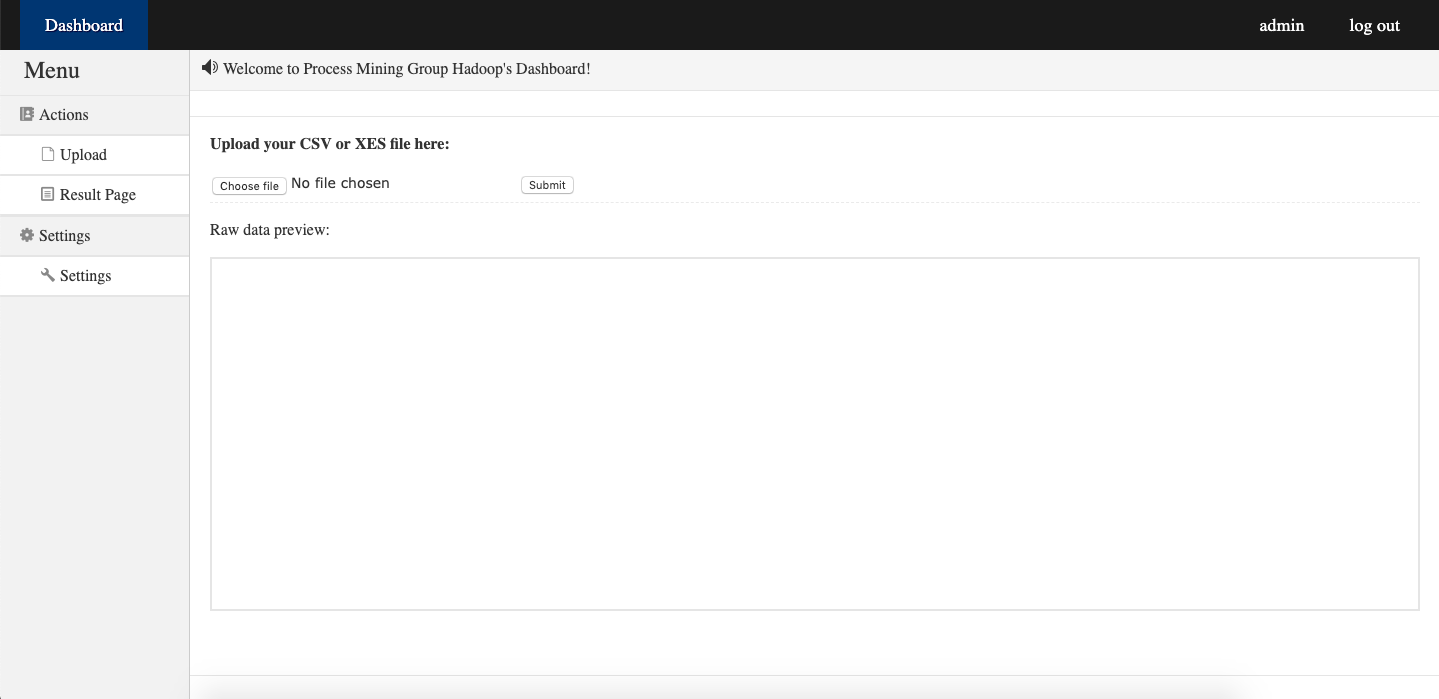
\includegraphics[scale=0.24]{dashboard.png}
	\caption{}
	\label{fig:label}
\end{figure}
\noindent
The main areas are:\\

\noindent
\textbf{1. Shortcut Bar} contains shortcuts to the dashboard site itself on the left side. The user settings and logout button can be found on the right side of the shortcut bar.\\\\
\noindent
\textbf{2. Main Toolbar} contains buttons with the most important functions for each applications like uploading the required files and the result page.\\\\
\noindent
\textbf{3. Main Window} displays the main content of the application. On the upload page there are upload bar and raw data preview box. After selected the file of right format, the content of the uploading file will be showed in the box.

\section{Installation}
The version control of this project depends on Git, and our team chose to use GitHub to manage our source code and releases.\\\\
\noindent
To deploy our WebApp on a server, you can just go to our GitHub releases page (\textit{https://github.com/xianganc/PraktikumProcessMining/releases}), then download the \textit{setup.sh} to local, run the contents inside the .sh file like in Fig. 2.

\begin{figure}[h]	
	\centering
	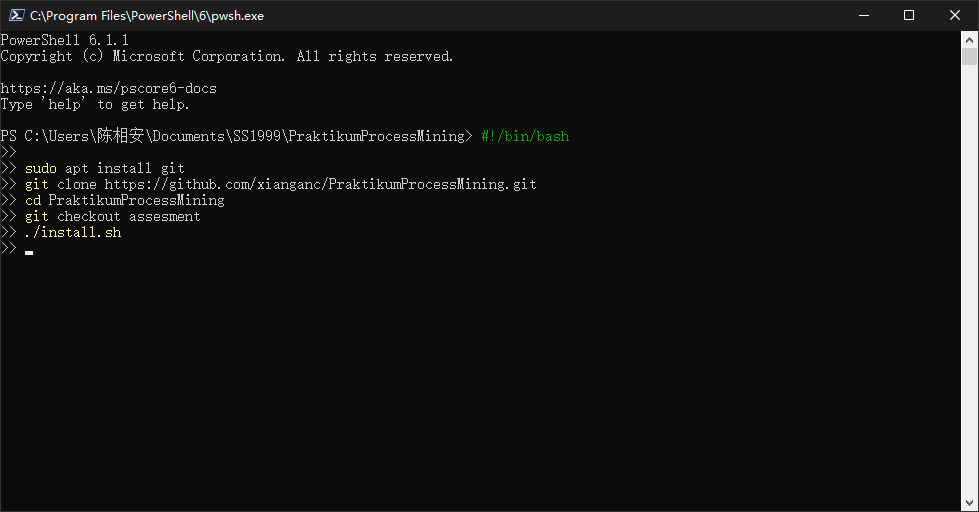
\includegraphics[scale=0.3]{setup.png}
	\caption{}
	\label{fig:label}
\end{figure}

\section{Upload}

In this section we explain how to use the WebApp. After reading this section, you will be able to preview the to be uploaded data and upload a CSV or XES file to the server.

\subsection{Uploading a CSV or XES File}

1. Click the \textit{Choose file} button on the top part of the main window.\\\\
\noindent
2. To upload a CSV or XES file, choose the file from local disk.\\\\
\noindent
3. If the selected file's format matches the server requirements, you will see the data inside the file in the text box below.\\\\
\noindent
4. Press \textit{Submit} button to upload the file to the server for further calculation.

\subsection{Replace a wrong selected file}
If you unexpectedly select a wrong file, you can do the followings:\\\\
\noindent
\textbf{2.2.1 Wrong File Format\\}
If the selected file were in the wrong format (e.g. a pdf file), then a pop-up window will show up, to notify the user for choosing a wrong file like Fig. 3.\\
\begin{figure}[h]	
	\centering
	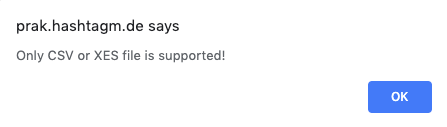
\includegraphics[scale=0.5]{wrong.png}
	\caption{}
	\label{fig:label}
\end{figure}

\noindent
\textbf{2.2.2 Wrong File Content\\}
If the selected file were with the wrong content, maybe the wrong selected has a similar file name as the should be seleted one. When the user selected a wrong file, you can re-select the file by clicking the \textit{Choose file} button or just refresh the website to re-select the file.

\section{Result}
After successfully submited the file, it should be uploaded to our server and being sent directly to calculation. 

\subsection{Check out the Output}
Then you can simply click the \textit{Result Page} on the left side in the main toolbar to check out the output.

\section{Log out}
If anytime the logged user want to log out, he can just click the \textit{logout} button on the top right corner to log out.

\end{document}
